\chapter{Introduction}
\label{chap:Introduction}

\section{Motivation}

Modern rail vehicles like trains, metro vehicles or trams have to meet ever increasing acoustic requirements and strict noise legislation not only to improve the acoustic comfort of the passengers, but also to reduce environmental noise pollution caused by railway transportation \cite{paozalyte_pollution_2011, li_25d_2021, zhang_sound_2019}.
% source of railway noise
A significant part of the train noise comes from the vehicle underfloor area where the bogies and auxiliary equipment, for example, the air supply system, the hydraulic system, or the electric system, are located. The major source of the underfloor noise is the rolling noise emitted by the wheel-rail interface at the bogie area. Besides that, for a driven bogie, the operational noise of traction motors also has a great contribution to the overall underfloor noise level.
% transmission of the underfloor noise
The airborne component of the bogie area noise (see \cref{fig:transmission_path}) on the one hand propagates directly into the exterior of the vehicle, disturbing the people in the surroundings, on the other hand, it could also be transmitted into the car interior for example through windows and doors, affecting the comfort of the passenger.
%
Hence, assessing the underfloor noise already in the early development phase of the rail vehicle is of great importance and can help in controlling the car exterior as well as the interior noise.


underfloor noise transmitted into the car interior as well as the exterior noise.



The transmission of noises is complex procedures because many paths: airborne, structure borne structural vibration


- outline the specific objective of the research
The aim of this thesis is ...

This thesis aims to provide/determine/develop/investigate

- Provide overview of thesis structure:
The thesis is structured as follow ...


\begin{figure}
    \centering
    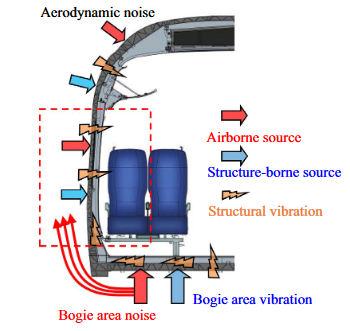
\includegraphics[width=0.5\textwidth]{fig/noise_transmission_path.png}
    \caption{Transmission path of exterior noise sources. Figure taken from \cite{zhang_sound_2019}.}
    \label{fig:transmission_path}
\end{figure}

\newpage
\section{Aims and objectives}

This thesis, in collaboration with Siemens Mobility Austria GmbH, aims to develop a finite-element model suitable for predicting the sound propagation from train underfloor area into the exterior environment around the carbody. 


The thesis is organised as follows. The fundamental background of the thesis is explained in Chap. \ref{chap:Theory}. Chap. \ref{chap:measurement} describes the outer pressure field measurement